\chapter{Planificación} \label{planificacion}
Para gestionar la planificación del proyecto, se ha implementado el método \textbf{Kanban} para organizar y asignar tareas de manera eficiente, utilizando la herramienta \textit{Wakatime} para registrar y analizar el tiempo invertido en cada actividad. Esta metodología permite un seguimiento preciso de las tareas completadas y del esfuerzo dedicado, asegurando así el cumplimiento de los objetivos semanales en un periodo de seis semanas. La planificación ha resultado fundamental para equilibrar el desarrollo del trabajo de fin de grado junto con las prácticas en la empresa, en las cuales dedico cinco horas diarias de trabajo durante la semana, dejando las tardes de entre semana y el fin de semana como el principal período de dedicación al proyecto académico.

\section{Planificación semanal}
Dado el marco temporal de seis semanas para la realización del proyecto, la planificación se ha dividido estratégicamente para asegurar un progreso constante y alcanzar los objetivos propuestos. A continuación, se detalla el enfoque semanal:

\begin{itemize}
    \item \textbf{Semana 1}: Revisión de la documentación y evaluación del estado del proyecto, definiendo prioridades y organizando las tareas iniciales.
    \item \textbf{Semana 2}: Resolución de \Gls{deuda} mediante la optimización y refactorización del código, mejorando la estabilidad y eficiencia del proyecto.
    \item \textbf{Semana 3}: Diseño y desarrollo de la interfaz de usuario, asegurando su integración con el backend y realizando pruebas de usabilidad.
    \item \textbf{Semanas 4 y 5}: Redacción de la memoria del TFG, incluyendo revisión, corrección y documentación de todo el trabajo realizado.
    \item \textbf{Semana 6}: Implementación de funcionalidades adicionales, realización de pruebas finales y ajustes, y finalización de la memoria para su entrega.
\end{itemize}
Cada semana de trabajo incluirá:
\begin{itemize}
    \item Organización de tareas mediante el tablero Kanban.
    \item Registro detallado de las horas invertidas en cada actividad, utilizando Wakatime.
    \item Consulta de literatura relevante y referencias empleadas para respaldar las decisiones tomadas.
    \item Registro de commits en GitHub, documentando los cambios significativos realizados (si aplica).
\end{itemize}

\begin{figure}[ht]
    \centering
    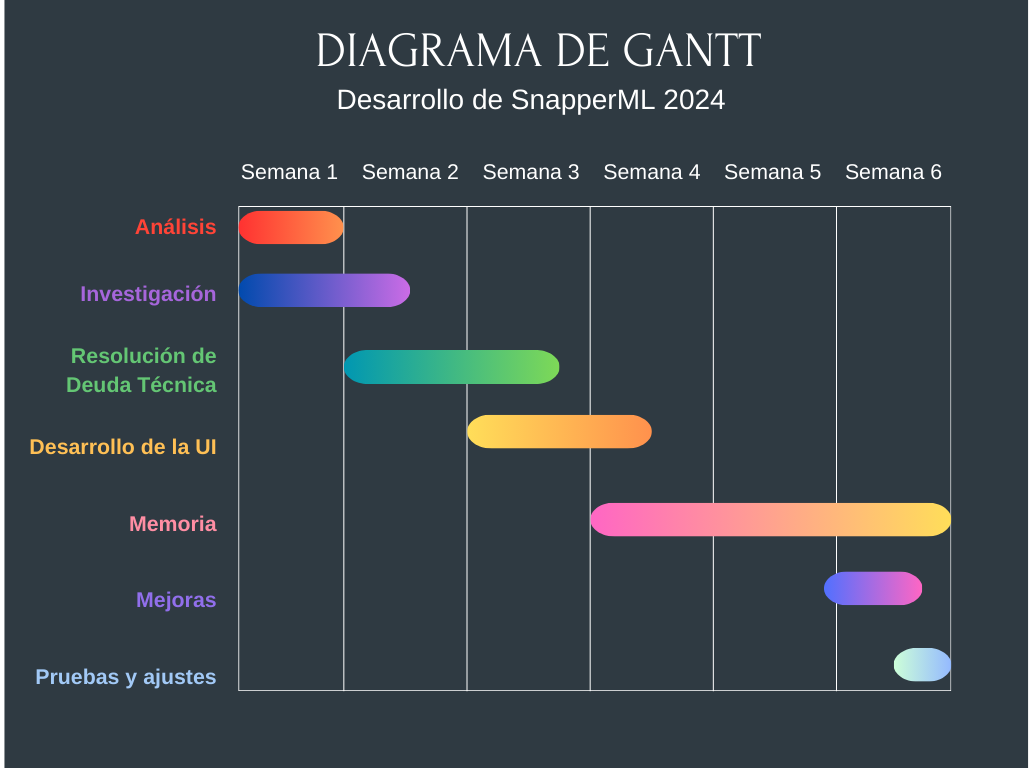
\includegraphics[width=0.9\textwidth]{imagenes/Gantt.png}
    \caption{Diagrama de Gantt del desarrollo de SnapperML.}
\end{figure}

\section{Semana 1: Documentación y prueba del estado del proyecto}
En la primera semana, se dedicará tiempo a la comprensión profunda del proyecto, evaluando su estado actual y revisando la documentación existente para identificar posibles problemas técnicos y áreas de mejora.

\subsubsection{Tareas de la semana}
\begin{itemize}
    \item Revisión de la estructura del proyecto y código existente.
    \item Leer la documentación actual del proyecto.
    \item Identificación de áreas con \Gls{deuda} para su futura resolución.
    \item Configuración de herramientas de seguimiento (Kanban y Wakatime). \item Revisión de literatura sobre \Gls{mlopsg} y buenas prácticas de desarrollo de software.
\end{itemize}

\subsubsection{Wakatime semanal}
Reporte semanal del tiempo de trabajo y análisis. Se ha trabajado principalmente con python.
\begin{figure}[h]
    \centering
    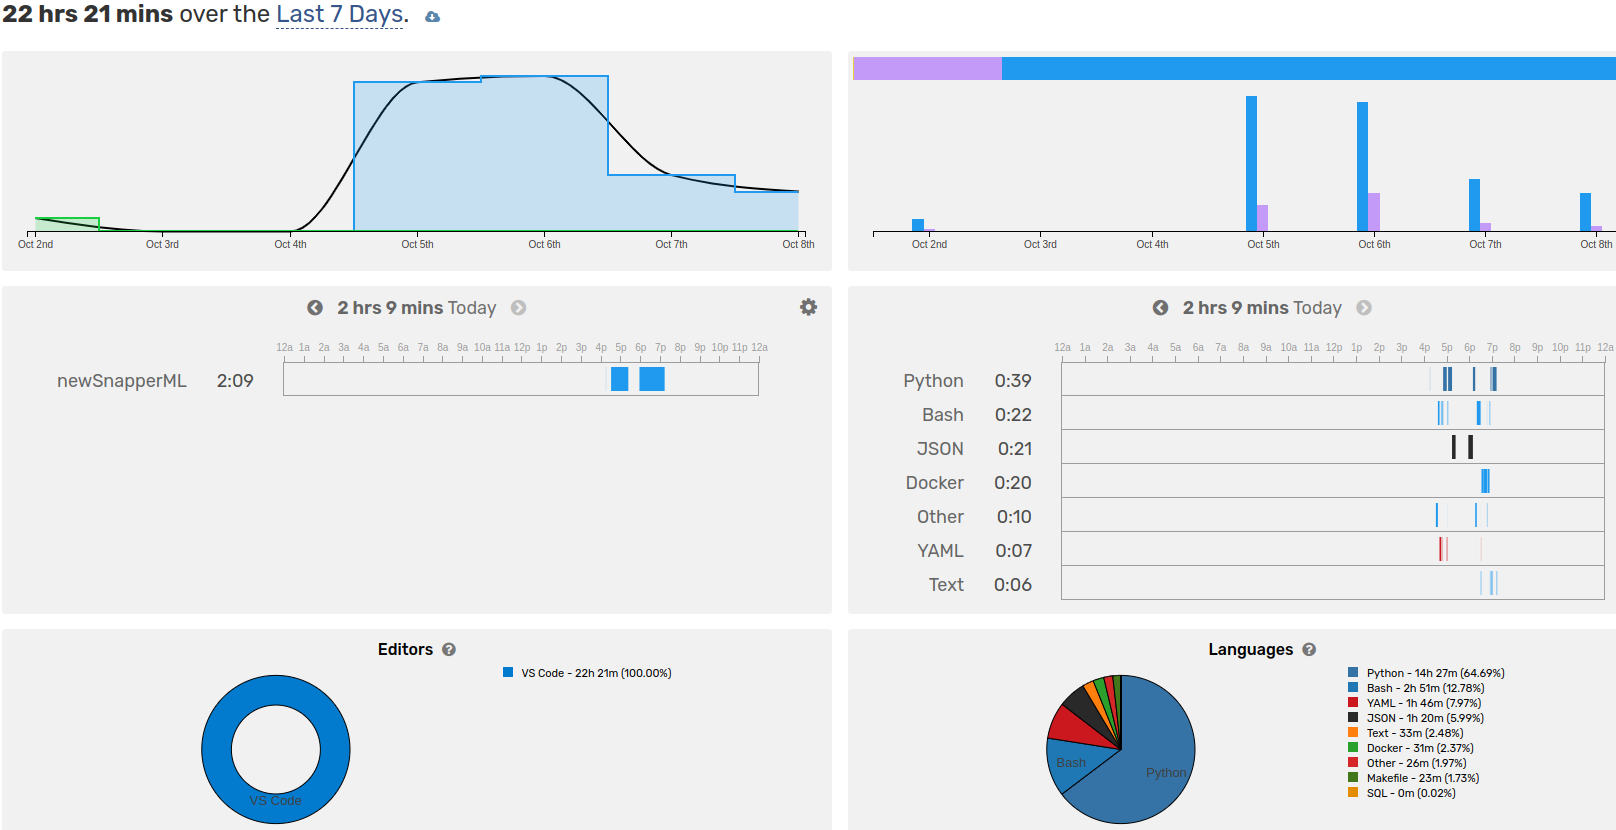
\includegraphics[width=\textwidth]{imagenes/wakatime_02-10_08-10.png}
    \caption{Registro de tiempo trabajado desde 02/10/2024 hasta 08/10/2024 según Wakatime.}
\end{figure}

Los días anteriores al 5 de Octubre fueron dedicados a realizar las primeras tareas de investigación y documentación. El navegador no está configurado con wakatime por eso no hay seguimiento.

\subsubsection{Literatura investigada}
\begin{itemize}
    \item \cite{mlops} \Gls{mlopsg}: buenas prácticas y fundamentos.
    \item \cite{introtodebt} Introducción al concepto de \Gls{deuda}.
    \item \cite{DORA} Informe DORA sobre \Gls{mlopsg}.
    \item \cite{snapperml_thesis} Tesis del ml-experiment realizada por Antonio Molner.
    \item \cite{snapperml_documentation} Documentacion oficial del \gls{framework} \Gls{snapperml}.
\end{itemize}

\section{Semana 2: Resolución de Deuda Técnica}
Durante la segunda semana, el enfoque se centrará en identificar y corregir la \Gls{deuda} acumulada en el proyecto, aplicando buenas prácticas de programación para optimizar la calidad y mantenibilidad del código. Las tareas planificadas incluyen:

\begin{itemize}
    \item Refactorización de módulos con código duplicado o excesivamente complejo.
    \item Migración y actualización de dependencias a sus versiones más recientes. \item Eliminación de código obsoleto o innecesario para simplificar la base de código.
    \item Optimización de funciones clave para mejorar el rendimiento general del sistema. \item Documentación detallada de los cambios realizados, incluyendo la justificación técnica de cada decisión.
\end{itemize}

Este enfoque contribuirá a un entorno de desarrollo más limpio y eficiente, facilitando futuras expansiones y mantenimientos.

\subsubsection{Kanban semanal}
Lista de tareas por tipo. Se muestra el tablero según el tipo de tarea que puede ser: Bug, Mejora (Enhancement) o Funcionalidad (Feature). Ver figura \ref{fig:kanban_deuda}.
\begin{figure}[ht]
    \centering
    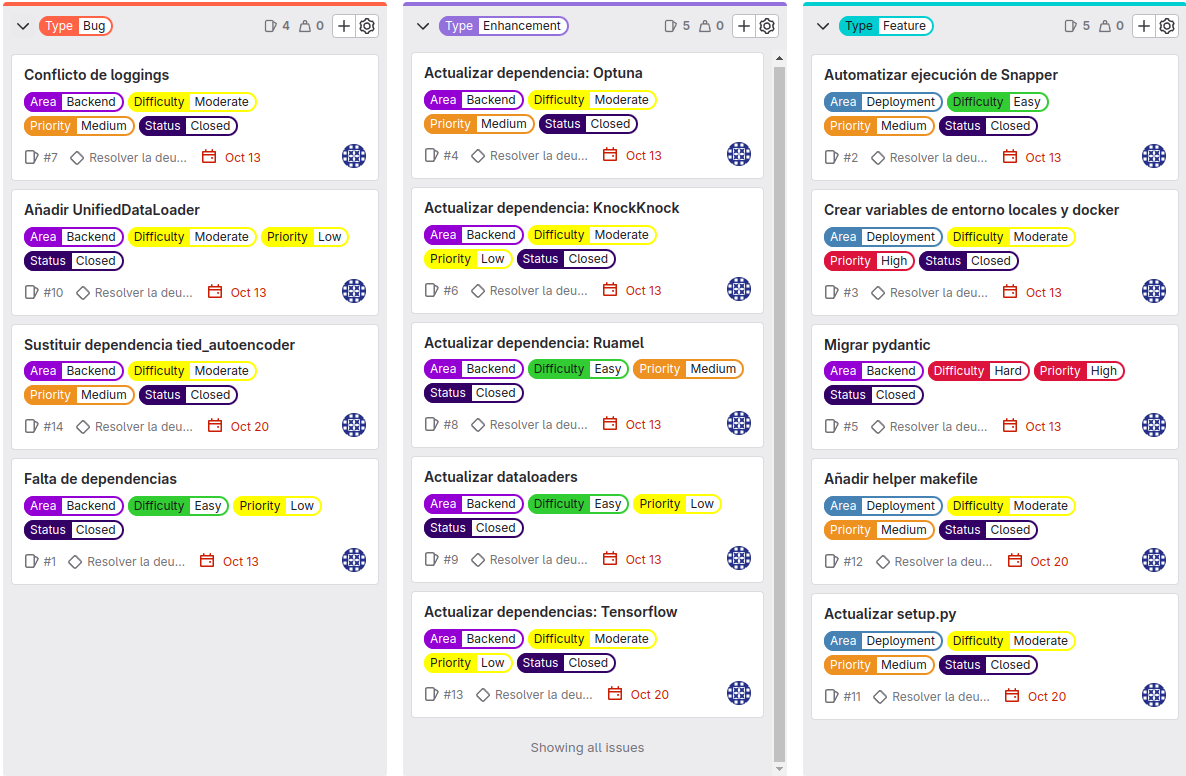
\includegraphics[width=\textwidth]{imagenes/kanban_resolver_deuda_tecnica.png}
    \caption{Tablero Kanban correspondiente al hito: Resolución de la \Gls{deuda}.}
    \label{fig:kanban_deuda}
\end{figure}

\subsubsection{Wakatime semanal}
Reporte semanal del tiempo de trabajo y análisis. Se trabaja principalmente con python. Ver figura \ref{fig:wakatime_07_10_2024} en la siguiente página.
\begin{figure}[H]
    \centering
    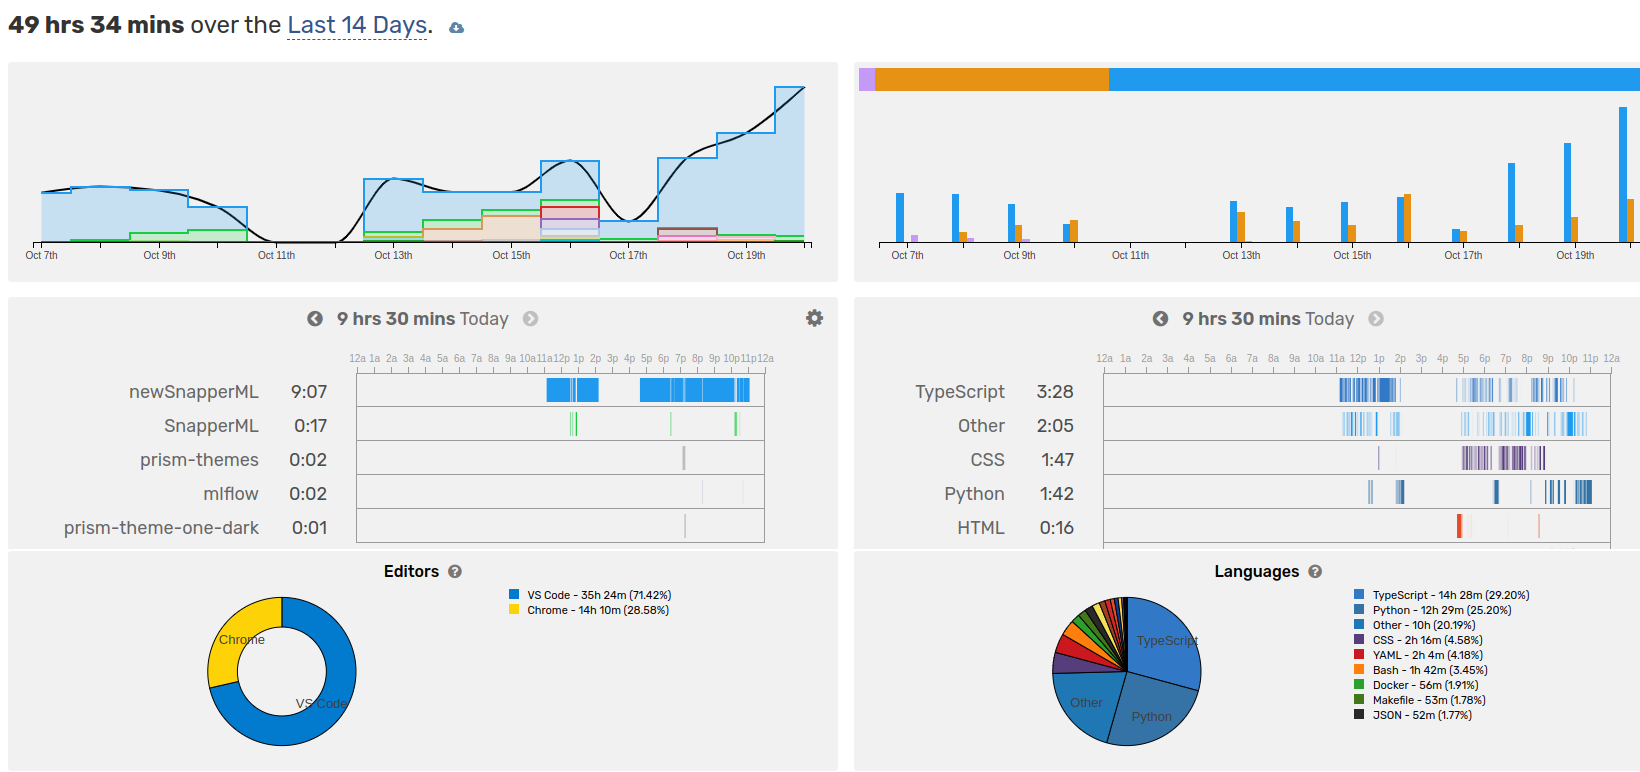
\includegraphics[width=\textwidth]{imagenes/wakatime_07-10_20-10.png}
    \caption{Registro de tiempo trabajado desde 07/10/2024 hasta 20/10/2024 según Wakatime.}
    \label{fig:wakatime_files_07_10_2024}
\end{figure}
\begin{figure}[H]
    \centering
    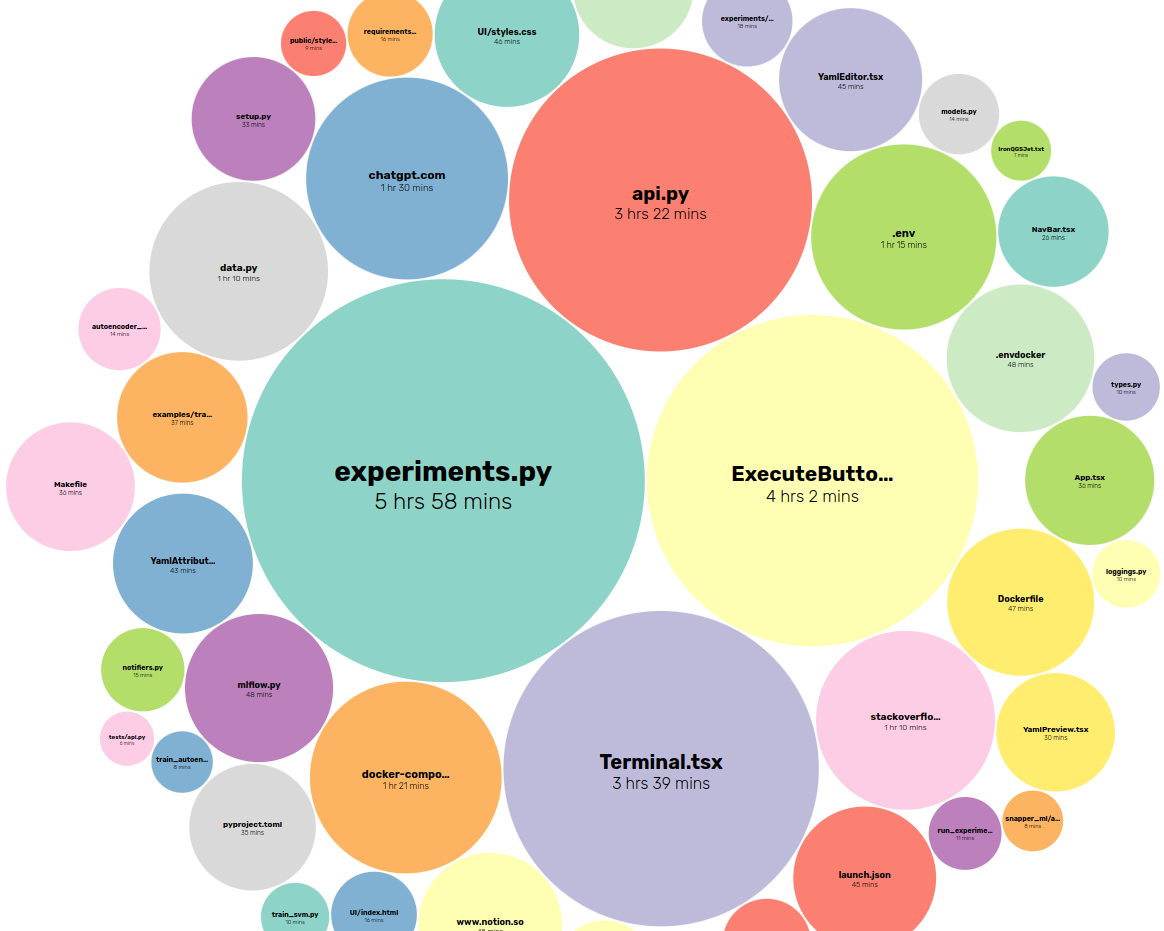
\includegraphics[width=.7\textwidth]{imagenes/wakatime_files_07-10_20-10.png}
    \caption{Registro de tiempo por archivos desde 07/10/2024 hasta 20/10/2024 según Wakatime.}
    \label{fig:wakatime_07_10_2024}
\end{figure}
\subsubsection{Commits}
Para un mejor seguimiento y organización se ha realizado un \say{pull request} al repositorio principal de \Gls{snapperml}.
\begin{figure}[H]
    \centering
    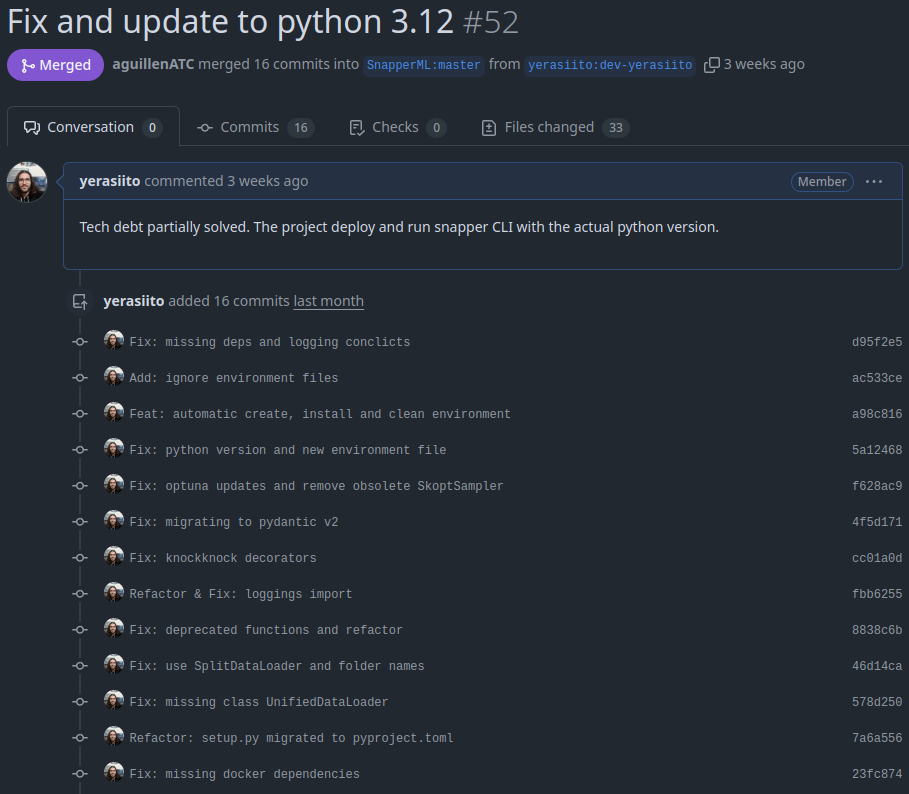
\includegraphics[width=\textwidth]{imagenes/github_pr_deuda.png}
    \caption{Pull request: Resolución de la \Gls{deuda}.}
    \label{fig:github_pr_deuda}
\end{figure}

\subsubsection{Literatura y recursos utilizados}
\begin{itemize}
    \item \cite{cunningham} Artículo de Ward Cunningham sobre \Gls{deuda}.
    \item \cite{introtodebt} Conceptos y gestión de \Gls{deuda}.
    \item \cite{stackoverflow_python_debug} Post de stackoverflow sobre como hacer debug en \acrshort{vsc}.
    \item \cite{pydantic} Dependencia de validación de configuración de los experimentos.
    \item \cite{mlops_principles} Principios fundamentales de \Gls{mlopsg}.
    \item \cite{knockknock} Dependencia de notificaciones.
    \item \cite{optuna_samplers} Dependencia de \acrfull{hpo}.
\end{itemize}

\section{Semana 3: Desarrollo de la interfaz de usuario}
Durante la tercera semana, se dedicará un esfuerzo significativo al diseño y desarrollo de una interfaz de usuario que no solo sea funcional, sino también intuitiva y atractiva para el usuario final. Se aplicarán principios de usabilidad y accesibilidad, asegurando que la interacción con el sistema sea sencilla para una amplia variedad de usuarios. Además, se buscará garantizar que la interfaz sea responsiva y se adapte adecuadamente a diferentes dispositivos y tamaños de pantalla, brindando una experiencia consistente y agradable.

\subsubsection{Tareas planificadas}
\begin{itemize}
    \item \textbf{Diseño de los componentes principales de la interfaz}, como formularios, botones y la visualización de \glspl{log}, garantizando una experiencia de usuario fluida.
    \item \textbf{Implementación de la interfaz empleando React y Bootstrap} para asegurar un desarrollo eficiente y un diseño moderno y responsivo. \item \textbf{Integración de la interactividad necesaria en la interfaz web}, optimizando la comunicación con el backend. \item \textbf{Creación de una API en Flask} que permita la comunicación entre el frontend y el backend.
    \item \textbf{Configuración y prueba de la responsividad de la interfaz} en distintos dispositivos y tamaños de pantalla, asegurando una visualización óptima.
    \item \textbf{Pruebas de usabilidad con usuarios de prueba}, recopilando comentarios y ajustando la interfaz para mejorar la experiencia de usuario.
    \item \textbf{Documentación completa de la estructura, funcionalidades y decisiones de diseño de la interfaz}, facilitando futuras mejoras y mantenimientos.
\end{itemize}

Este enfoque garantizará que la interfaz sea intuitiva y fácil de usar, proporcionando una experiencia visualmente atractiva que capte la atención del usuario y se mantenga coherente con los objetivos generales del proyecto.

\subsubsection{Kanban semanal}
Lista de tareas por tipo. Se muestra el tablero según el tipo de tarea que puede ser: Bug, Mejora (Enhancement) o Funcionalidad (Feature). Ver figura \ref{fig:kanban_desarrollar_la_interfaz_web} en la página siguiente.
\begin{figure}[ht]
    \centering
    \includegraphics[width=\textwidth]{imagenes/kanban_desarrollar_la_interfaz_web.png}
    \caption{Tablero Kanban correspondiente al hito: Desarrollar la Interfaz Web.}
    \label{fig:kanban_desarrollar_la_interfaz_web}
\end{figure}

\subsubsection{Wakatime semanal}
Reporte semanal del tiempo de trabajo y análisis.
\begin{figure}[H]
    \centering
    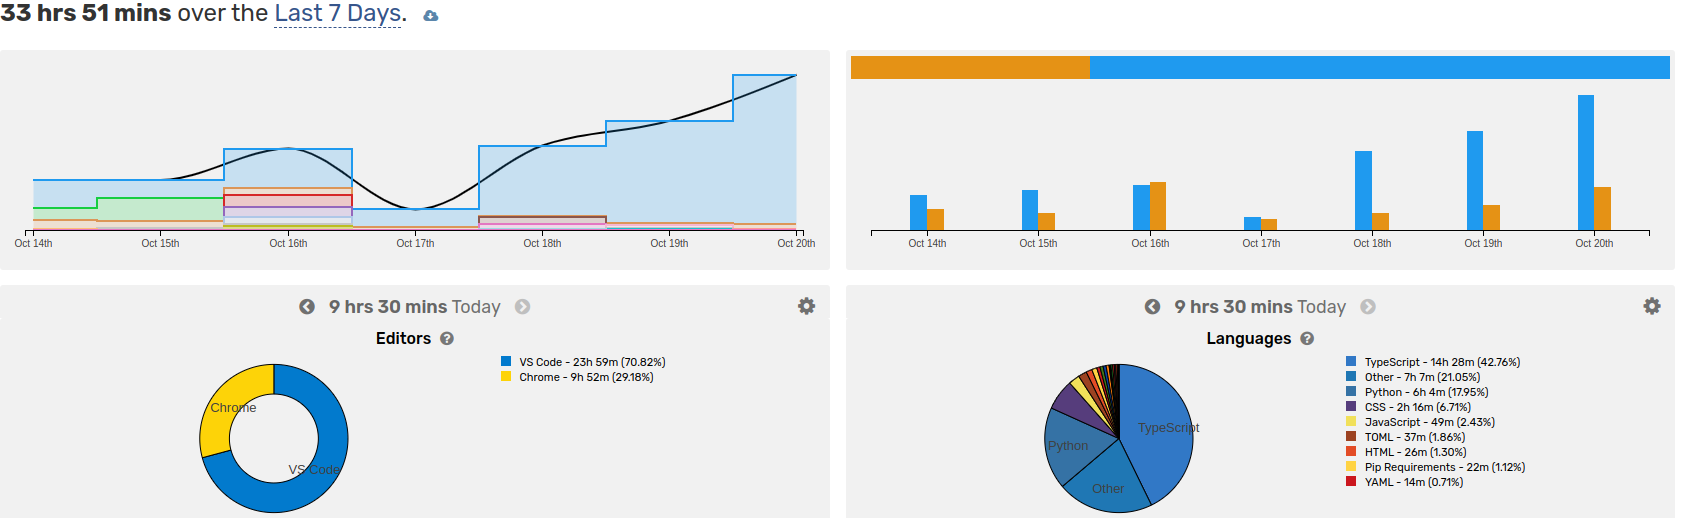
\includegraphics[width=\textwidth]{imagenes/wakatime_14-10_20-10.png}
    \caption{Registro de tiempo trabajado desde 14/10/2024 hasta 20/10/2024 según Wakatime.}
\end{figure}
Tiempo record de 9 horas y 30 minutos el Domingo 20 de Octubre con aumento del 169\% de la productividad.

\subsubsection{Commits}
Para un mejor seguimiento y organización se ha realizado un \acrfull{pr} al repositorio principal de \Gls{snapperml}. Ver figura \ref{fig:github_pr_ui}.

\begin{figure}[H]
    \centering
    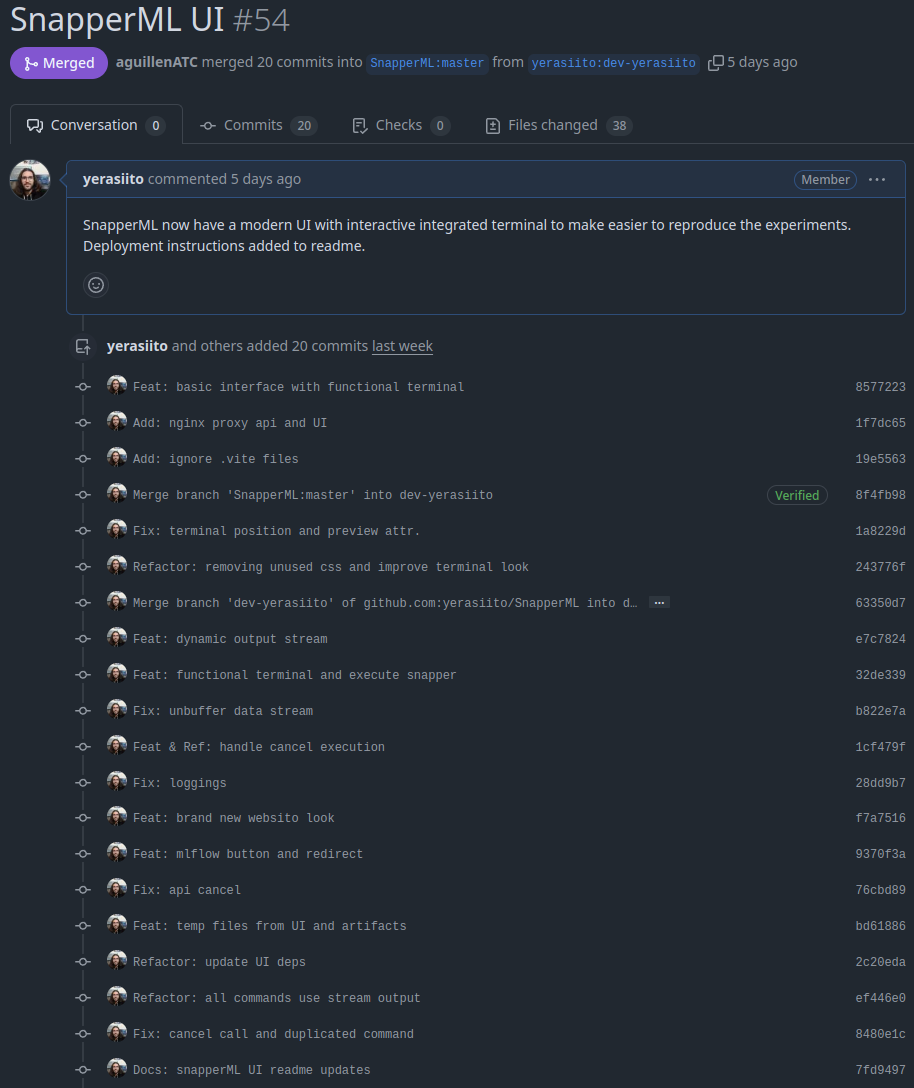
\includegraphics[width=0.95\textwidth]{imagenes/github_pr_ui.png}
    \caption{\acrlong{pr}: \Gls{snapperml} UI.}
    \label{fig:github_pr_ui}
\end{figure}

\subsubsection{Literatura y recursos utilizados}
\begin{itemize}
    \item \cite{reactdocs} Documentación de React.
    \item \cite{bootstrap} Documentación de Bootstrap.
    \item \cite{vite} ¿Por qué elegir vite?
    \item \cite{typescript} Handbook de typescript.
    \item \cite{cors} \acrfull{cors}
    \item \cite{flask} Pagina oficial de Flask (\Gls{apig})
\end{itemize}

\section{Semana 4 y 5: Redacción de la memoria}
Durante la cuarta y quinta semana, el objetivo principal será progresar de manera significativa en la redacción de la memoria del proyecto. Se documentarán en detalle todos los aspectos técnicos y funcionales, abarcando desde la planificación y el diseño hasta la implementación y las pruebas realizadas. Además, se describirá el proceso de desarrollo de manera estructurada, proporcionando un análisis claro de las decisiones técnicas tomadas y su justificación, junto con las dificultades encontradas y cómo se resolvieron. Esto asegurará una memoria completa y comprensible, que refleje fielmente el trabajo realizado.

\subsubsection{Tareas de la semana}
\begin{itemize}
    \item Redacción de la sección de introducción y objetivos del proyecto.
    \item Documentación de los requisitos y la especificación del sistema.
    \item Descripción detallada de las soluciones aplicadas para resolver la \Gls{deuda}.
    \item Redacción de la planificación semanal y metodología.
    \item Redacción de la implementación y conclusiones.
\end{itemize}
Se dedicará especial atención a mantener una redacción clara y coherente, asegurando que cada sección de la memoria aporte valor y esté adecuadamente estructurada. Además, se emplearán gráficos, tablas y ejemplos de código donde sea necesario para ilustrar conceptos complejos y facilitar la comprensión. La memoria final buscará no solo cumplir con los requisitos académicos, sino también servir como un recurso de referencia útil para futuros desarrolladores o investigadores interesados en el proyecto.

\subsubsection{Kanban semanal}
Lista de tareas por prioridad. A continuación se muestra el tablero kanban según la prioridad de la tarea: baja, media o alta.
\begin{figure}[ht]
    \centering
    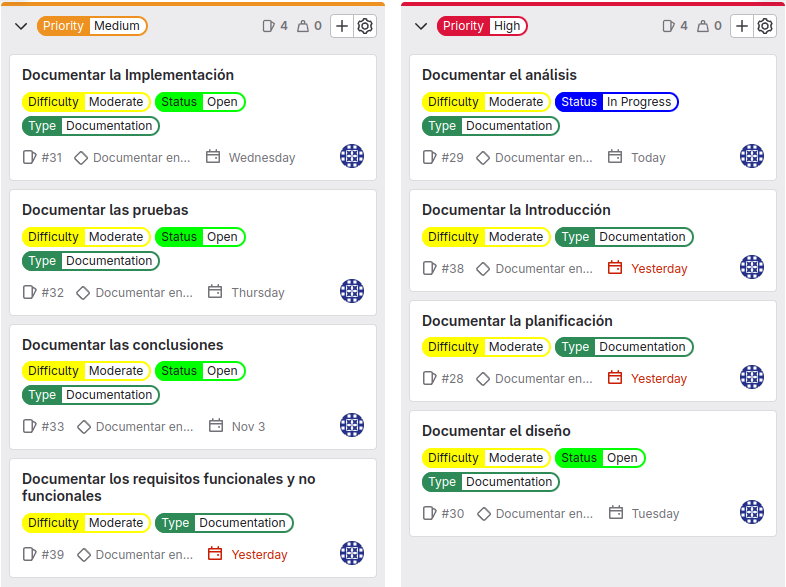
\includegraphics[width=0.87\textwidth]{imagenes/kanban_documentar_la_memoria.png}
    \caption{Tablero Kanban correspondiente al hito: Documentar la memoria.}
\end{figure}

\subsubsection{Wakatime semanal}
\vspace{-0.5em}
\begin{figure}[H]
    \centering
    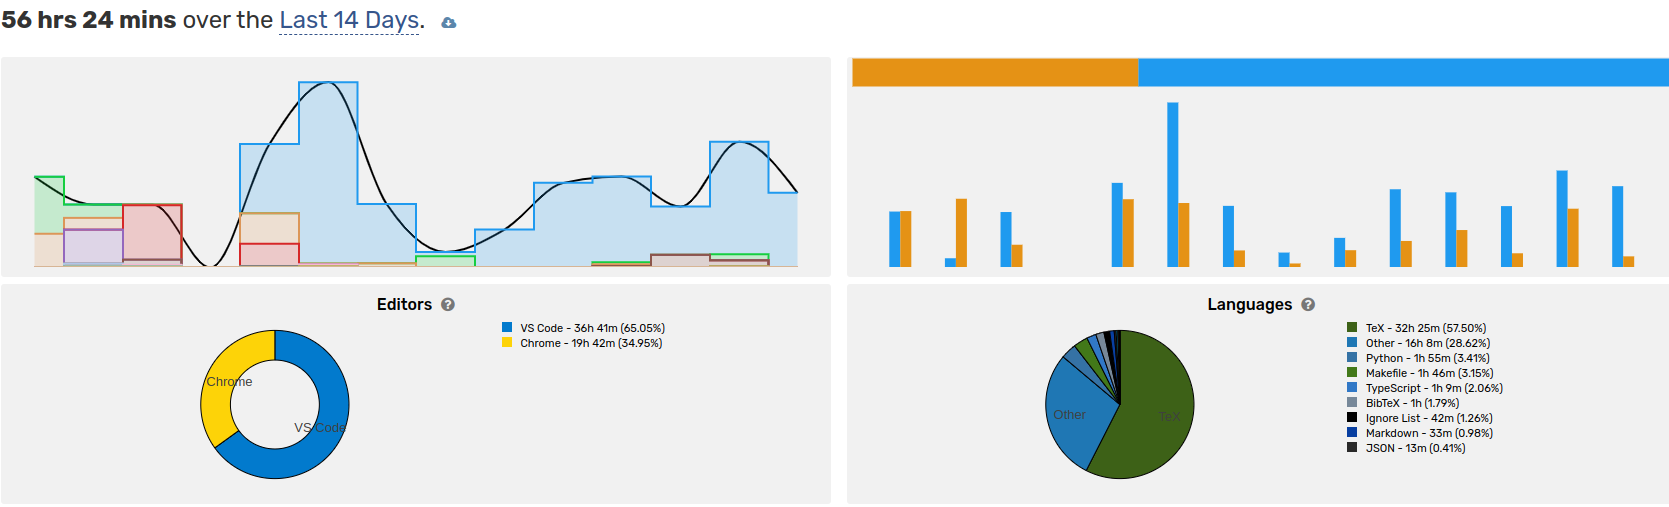
\includegraphics[width=\textwidth]{imagenes/wakatime_22-10_04-11.png}
    \caption{Registro de tiempo trabajado desde 22/10/2024 hasta 03/11/2024 según Wakatime.}
\end{figure}

\subsubsection{Literatura utilizada}
\begin{itemize}
    \item Documentación interna del proyecto.
    \item Cualquier fuente citada en el TFG, para una referencia precisa en el documento.
\end{itemize}


\section{Semana 6: Funcionalidades adicionales y lanzamiento}
La sexta semana marca un hito crucial en el desarrollo del proyecto, enfocándose en la adición de funcionalidades finales, la estabilización del código, y el empaquetado del framework para su distribución oficial. El objetivo principal de esta etapa es preparar SnapperML para su lanzamiento en la plataforma PyPI, lo que permitirá a los usuarios descargar e instalar el paquete de manera sencilla, facilitando así su uso y adopción.

\subsubsection{Tareas de la semana}
\begin{itemize}
    \item Implementación de funcionalidades adicionales solicitadas por el tutor.
    \item Creación de pruebas unitarias y de integración para el nuevo código.
    \item Actualización de la documentación con las nuevas funcionalidades y pruebas.
    \item Empaquetado y lanzamiento del paquete en PyPI.
    \item Validación de la accesibilidad de la interfaz para usuarios con diferentes necesidades.
    \item Revisión final de toda la documentación del proyecto.
\end{itemize}
\subsubsection{Kanban semanal}
Lista de tareas por tipo. Se muestra el tablero según el tipo de tarea que puede ser: Bug, Mejora (Enhancement) o Funcionalidad (Feature). Ver figura \ref{fig:kanban_mejorar_snapper}

\begin{figure}[H]
    \centering
    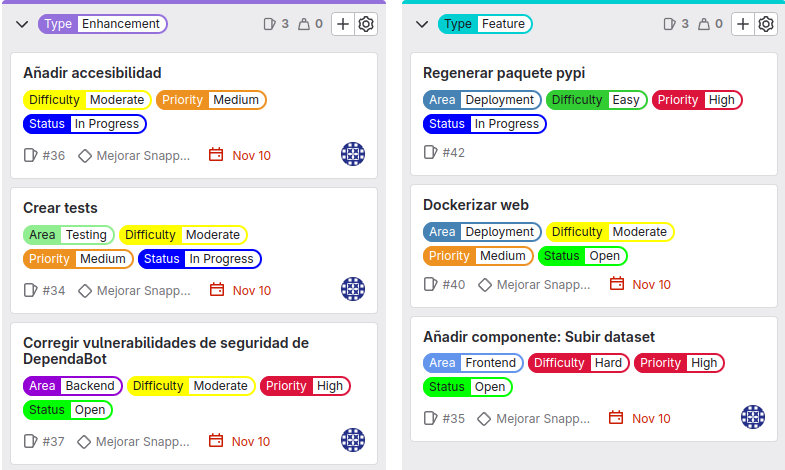
\includegraphics[width=0.88\textwidth]{imagenes/kanban_ampliar_snapper.png}
    \caption{Tablero Kanban correspondiente al hito: Mejorar snapperML.}
    \label{fig:kanban_mejorar_snapper}
\end{figure}

\subsubsection{Wakatime semanal}
\begin{figure}[h]
    \centering
    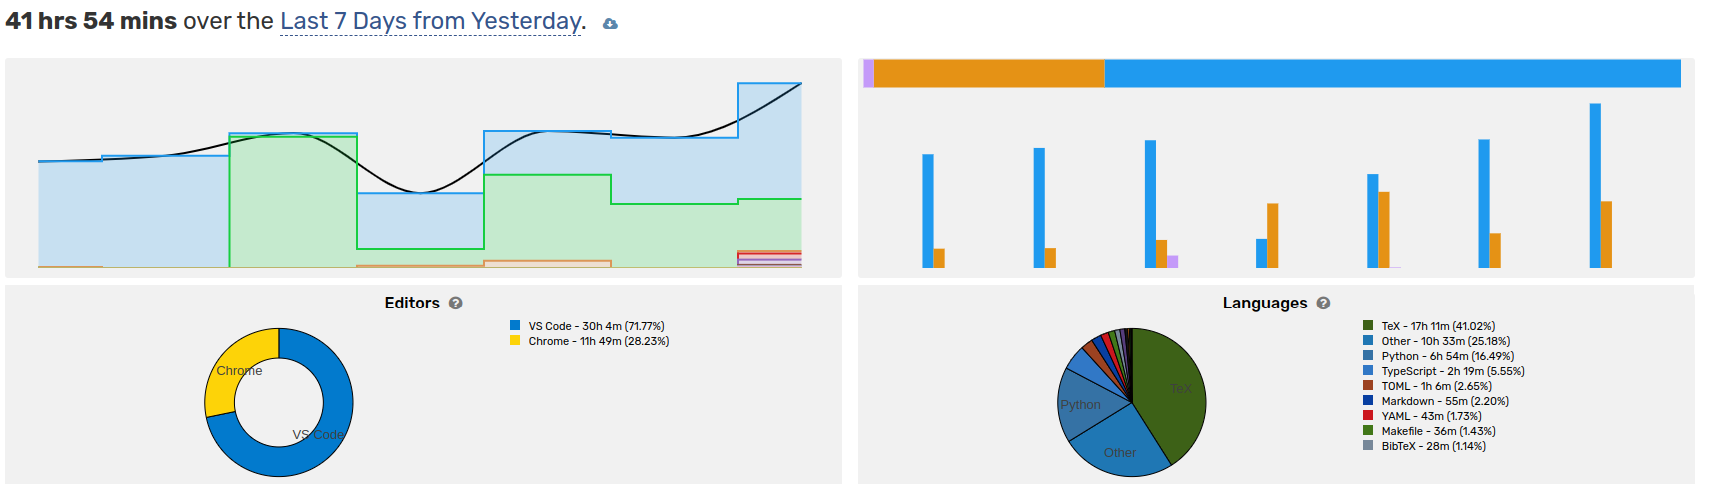
\includegraphics[width=\textwidth]{imagenes/wakatime_04-11_10-11.png}
    \caption{Registro de tiempo trabajado desde 04/11/2024 hasta 10/11/2024 según Wakatime.}
\end{figure}

\subsubsection{Literatura utilizada}
\begin{itemize}
    \item Referencias adicionales sobre \Gls{mlopsg} y diseño de pruebas en proyectos de software.
    \item \cite{security} Guías sobre seguridad en desarrollo web.
    \item \cite{accesibilidad_espania} Guías de accesibilidad y usabilidad para interfaces web.
\end{itemize}

\section{Presupuesto}
El presupuesto del desarrollo se ha estimado considerando no solo la duración de las diferentes tareas, sino también el tiempo y esfuerzo invertidos de manera continua a lo largo del proyecto. Cabe destacar que, a pesar de compaginar las exigencias del Trabajo de Fin de Grado (TFG) con las prácticas en la empresa, se ha logrado mantener un ritmo de trabajo eficiente y constante. Para el cálculo del presupuesto, se han tenido en cuenta los siguientes elementos clave:

\begin{itemize}
    \item \textbf{Contribuciones a los repositorios de control de versiones}: Las plataformas de desarrollo colaborativo, como GitHub y GitLab, registran las contribuciones realizadas durante el año. Estas contribuciones incluyen implementaciones de nuevas funcionalidades, mejoras en el código, documentación, y ajustes necesarios para optimizar el framework y la memoria. El registro detallado de estas actividades proporciona un indicador tangible del esfuerzo y la dedicación invertidos.
          \begin{itemize}
              \item \textbf{Contribuciones en GitHub}: Se han realizado un total de 52 contribuciones relacionadas con el desarrollo del framework SnapperML, reflejando las implementaciones, mejoras y correcciones de código durante el desarrollo.
                    \begin{figure}[ht]
                        \centering
                        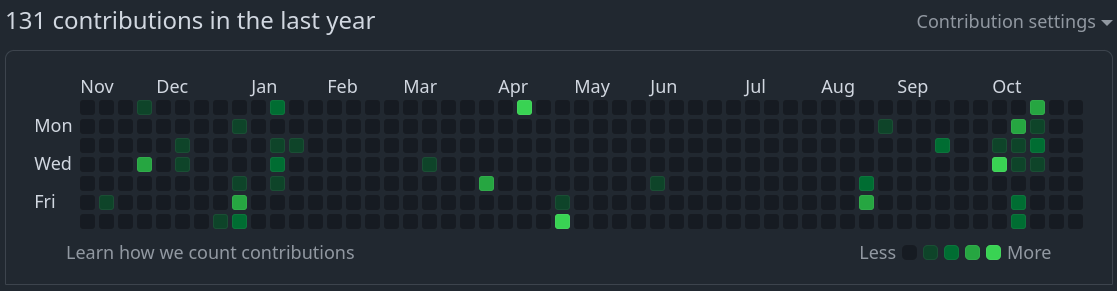
\includegraphics[width=0.85\textwidth]{imagenes/activity_github.png} \caption{Contribuciones a GitHub durante el año (52 a SnapperML).}
                    \end{figure}
              \item \textbf{Contribuciones en GitLab}: Se han registrado 101 contribuciones destinadas al desarrollo de tareas, la documentación y la elaboración de la memoria del TFG, mostrando un enfoque meticuloso en la organización y presentación del trabajo.
                    \begin{figure}[ht]
                        \centering
                        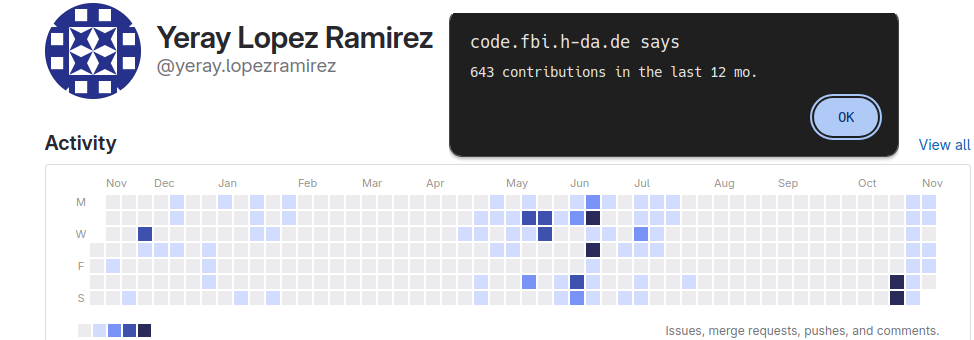
\includegraphics[width=0.9\textwidth]{imagenes/activity_gitlab.png}
                        \caption{Contribuciones a GitLab durante el año (101 a las tareas y la memoria).}
                    \end{figure}
          \end{itemize}
    \item \textbf{Registros de Wakatime}: Esta herramienta ha sido fundamental para monitorizar el tiempo dedicado al desarrollo activo. Las horas contabilizadas reflejan el trabajo directo en la codificación, depuración, y documentación técnica del proyecto, ofreciendo una base sólida para calcular el esfuerzo real en términos de tiempo.
    \item \textbf{Estimaciones de tareas complementarias}: Además del tiempo activo registrado por Wakatime, se ha estimado el tiempo necesario para tareas complementarias. Estas incluyen el diseño de diagramas, la investigación para fundamentar las decisiones técnicas, la asistencia a tutorías para recibir orientación, y la planificación estratégica de objetivos y tareas.
\end{itemize}

En la figura \ref{fig:presupuesto}, se resumen las horas totales dedicadas al desarrollo del proyecto, desglosadas en dos categorías: el tiempo registrado con Wakatime y las horas estimadas para tareas no directamente contabilizadas. Estas últimas incluyen actividades esenciales como la asistencia a tutorías, el diseño de elementos gráficos y diagramas, la planificación detallada de tareas y las búsquedas de información necesarias para fundamentar el proyecto y optimizar las decisiones de desarrollo.

El desarrollo del TFG ha requerido un total de 300 horas, que se distribuyen de la siguiente manera:
\begin{itemize}
    \item \textbf{Horas contabilizadas por Wakatime}: 204 horas y 22 minutos, que reflejan el tiempo de trabajo activo en el desarrollo de SnapperML y la documentación.
    \item \textbf{Horas estimadas}: 106 horas, dedicadas a actividades como tutorías, diseño gráfico, investigación documental y planificación detallada.
\end{itemize}

Para calcular el coste total del desarrollo, se ha tomado como referencia el salario promedio de un desarrollador Fullstack en España, que según la plataforma Glassdoor \cite{glassdoor} es de 11,54 € por hora. Con esta tarifa, el coste del desarrollo completo asciende a 3.581,63 €, lo que refleja la suma del tiempo activo registrado por Wakatime y las horas estimadas para tareas complementarias.

\begin{figure}[h]
    \centering
    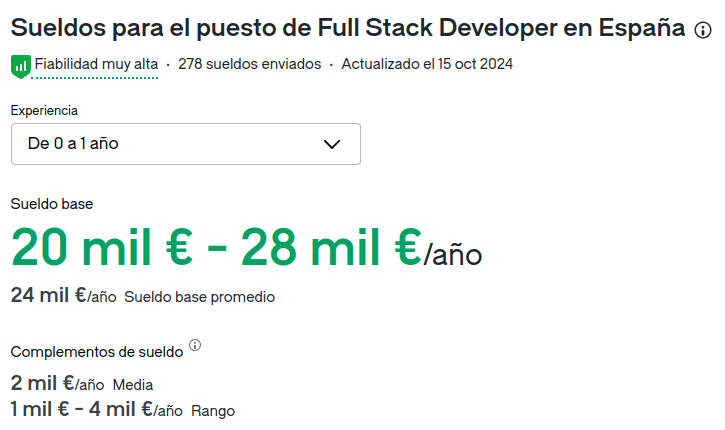
\includegraphics[width=0.7\textwidth]{imagenes/sueldo_fullstack.png}
    \caption{Sueldo medio de un Desarrollador Fullstack en España 2024 (11,54€/h).}
\end{figure}

Además, se incluye un gasto adicional de 500 € por el equipo necesario, en este caso, un ordenador Asus Vivobook D152DA, lo que eleva el coste total del desarrollo a 4.081,63 €.

\begin{figure}[h]
    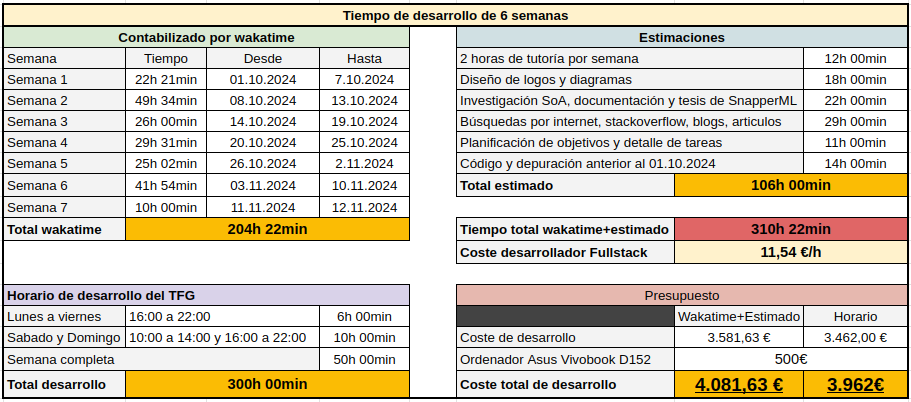
\includegraphics[width=\textwidth]{imagenes/total_horas.png}
    \caption{Presupuesto total.}
    \label{fig:presupuesto}
\end{figure}

De este modo, se concluye que se han cumplido las 300 horas requeridas para el desarrollo del TFG, asegurando una dedicación constante y estructurada para cumplir con los objetivos planteados.